%===============================================================================%
\section{Data processing} \label{section:processing}
%===============================================================================%

The sources of uncertainties in the Wi-Fi probe request data were discussed in detail in section \ref{section:uncertainties} and the major ones that were identified were - range of the sensor, probing frequency of the mobile devices, randomisation and hashing of MAC addresses, changing mobile ownership and missing data.
Out of this it was found that the MAC address collision occurring due to the hashing process was found to be insignificant could be ignored safely.
The missing data problem was found to be an issue of `post processing' where the values need to estimated based on the previously occurring values after the rest of the uncertainties are solved.
Which left MAC randomisation and uncertainty regarding the range of the sensors as the major sources of noise in the data.
The next step was to explore the extent of the noise generated by looking at the sample data collected and the real world data from Smart Street sensor project.

During the early stages of the Smart Street Sensor project, in 2015, a data quality audit was conducted to estimate the amount of noise in the data before moving to analysing them \cite{lugomer2017}.
A field survey was conducted at locations in Sheffield and London over 5 days in September and December 2016 and manual pedestrian counts were collected for these location to be compared to the counts reported by the sensors.
It was intuitively expected that there will be errors in the sensor collected data arising from various internal and external factors which may lead to the under-counting and over-counting at the chosen locations.
But since the MAC randomisation was introduced in iOS devices months before, it was also expected to be manageable with a standard adjustment factor which is a combined measure of ratios of the Apple devices which we observed in sensors prior to randomisations.
Surprisingly, the study found that even with fairly complicated adjustment factors the errors are large and unpredictable and emphasised our lack of detailed understanding of the probe request process.
The results showed that the errors vary between 16\% to -41\% within the same day and though an adjustment factor based on manual data collection reduces the errors to less than 5\% there was a risk of substantially under counting and over counting depending on the quality of the field survey.
The study also called for a more close look into the randomisation process and development of more advanced data mining methods to reduce the reliance on manual counting on the field leading to the motivations of this research.

\begin{marginfigure}
  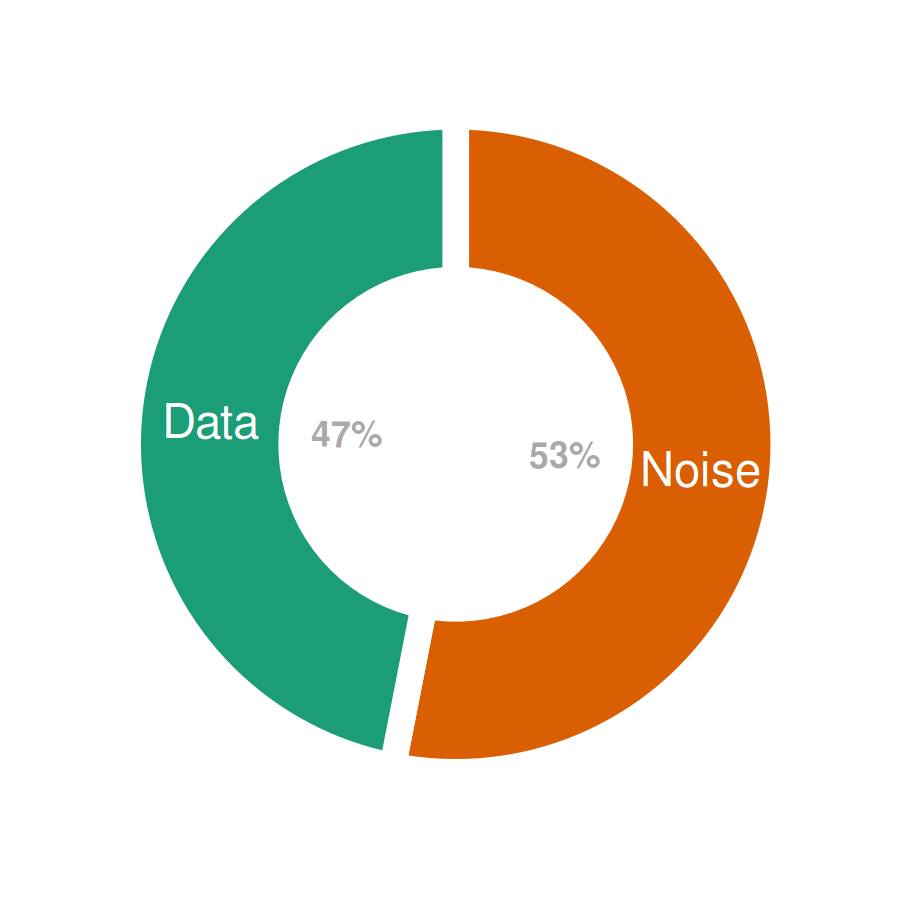
\includegraphics[trim={10 10 10 10 },clip]{images/processing-error-signal.png}
  \caption{The share of noise present in the data from outside the field of measurement in the initial experiment.}
  \label{figure:processing:error:signal}
\end{marginfigure}

From the initial experiment, the noise due to the uncertain range of sensors was found to be much larger than what was expected.
It was observed that about 53\% of the total probe requests collected were from the outside the desired field of study and the errors can be reduced massively just filtering out this noise as shown in Figure \ref{figure:processing:error:signal}.
It was noticed that the signal strength of the received probe requests gives us valuable information on whether the probe request is generated by a device within the field of study.
Moreover, the amount of noise generated was found to be much greater in the data collected in a more real world setting at UCL.
The experiment showed that the Mean Average Percentage Error when comparing the sensor counts to manual counts of pedestrians were reduced from 736\% to  80\% just by removing signal strengths which are lower than -70dBm.
The problem with that methodology is the arbitrary nature of the threshold -70dBm which can vary widely based on the site conditions and over time.
A robust method is needed to calculate this threshold dynamically for each location at a particular time which is derived from the data itself rather than requiring external sources of information such as regular field surveys.

As discussed in chapter \ref{chapter:literature} and \ref{chapter:collection} MAC randomisation is one of the major issue in the data which has been created as a result of the efforts to protect the privacy of the users of mobile devices which cannot be just eliminated by collecting more data.
The idea that we should protect the privacy of the users also eliminates most of the intrusive techniques for collecting and processing data.
The technique of randomising MAC has been used by Windows Operating system for a long time on laptop computers but it was brought to mainstream when Apple Inc. introduced iOS 8 for their mobile devices in the fall of the 2015.
It was observed that there was a massive wave of adoption shortly after the release but the trend stabilised as more and more market share was captured by Android devices which weren't randomising the MAC addresses at the time.
The trend has been remained stable until fall of 2017 even with Google phones switching to randomisation techniques. 
It is important to note that the randomisation methods were neither fool proof nor standardised as showed by \citep{vanhoef2016}.
The problem intensified massively in 2017 which could be attributed to the change in how many times MAC addresses were randomised in a given time interval thus increasing the proportion of local addresses all over the dataset along with the total number of unique addresses.

\begin{figure*}
  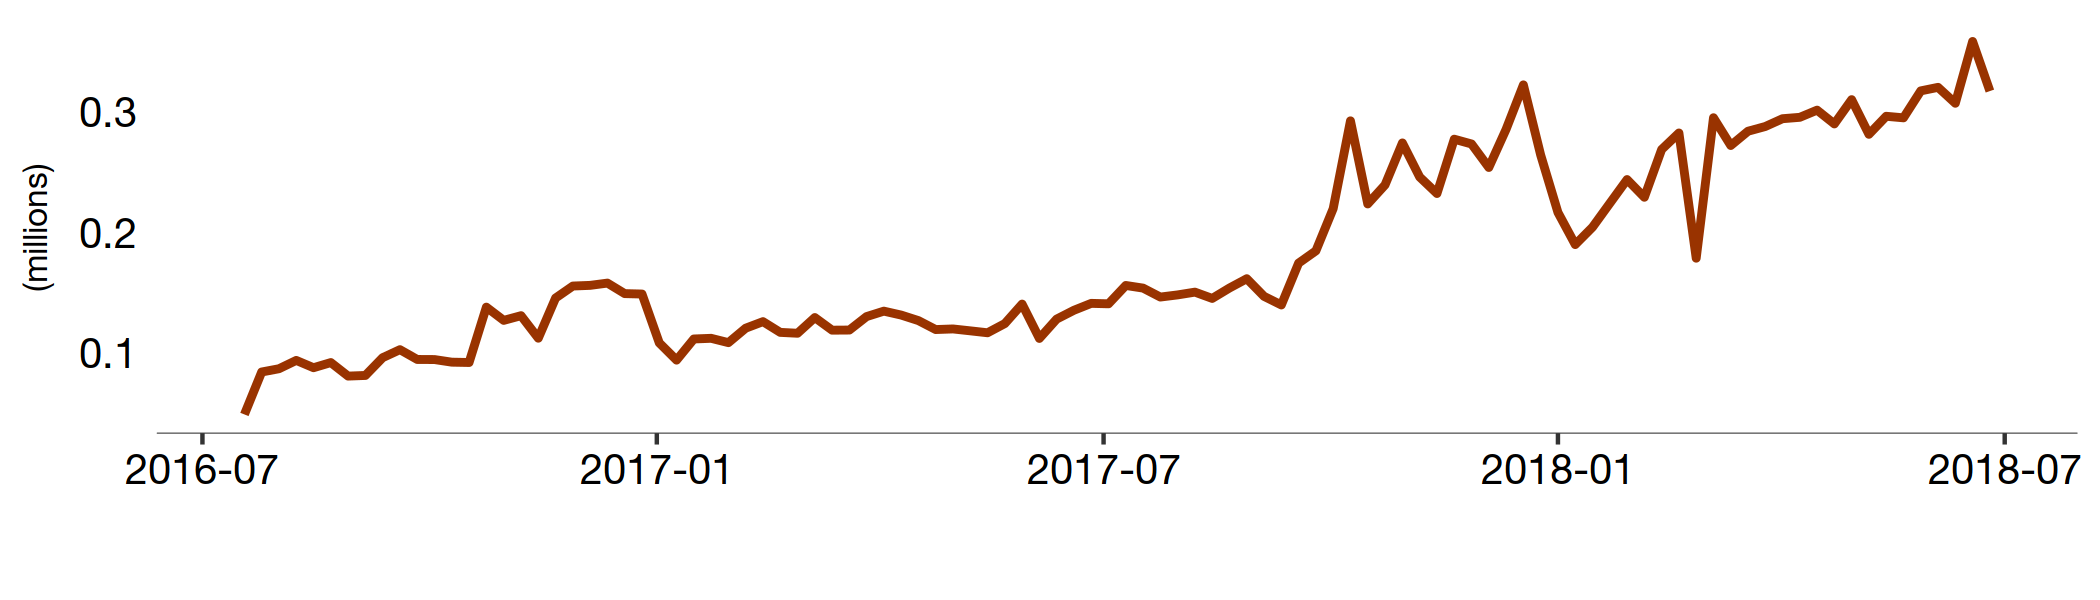
\includegraphics[trim={0 0 0 0},clip]{images/processing-error-randomisation.png}
  \caption{The share of noise present in the data from outside the field of measurement in the initial experiment.}
  \label{figure:processing:error:random}
\end{figure*}

Figure \ref{figure:processing:error:random} shows the resulting `explosion' average number of unique MAC addresses that occurred in September 2017 from a subset of data comprising of sensors at Cardiff.
Moreover it is not possible that that the overall increase in the unique MAC addresses cannot be due to the just the increase of footfall at these locations.

In addition to causing problems generally in the data for longitudinal analysis, randomisation also causes issues at specific locations which have potential for large amount of devices to dwell around them.
For example, seating areas in cafes/ restaurants, bus stops, phone shops around the sensors causes huge overestimation of footfall when aggregated by unique MAC addresses.
It is imperative that the method we device should take both these cases in to consideration.

%-------------------------------------------------------------------------------%
\subsection{Methodology}
%-------------------------------------------------------------------------------%
Keeping the above considerations in mind, we propose two methods to clean the Wi-Fi data and process them into footfall data.
The first method uses signal strengths to filter out the noise originating from outside the field of view and the second uses the sequence numbers to group probe requests together instead of MAC addresses.

\vspace{1.5em}\noindent\textit{Filtering with Signal Strength}\vspace{0.5em}

\begin{marginfigure}
  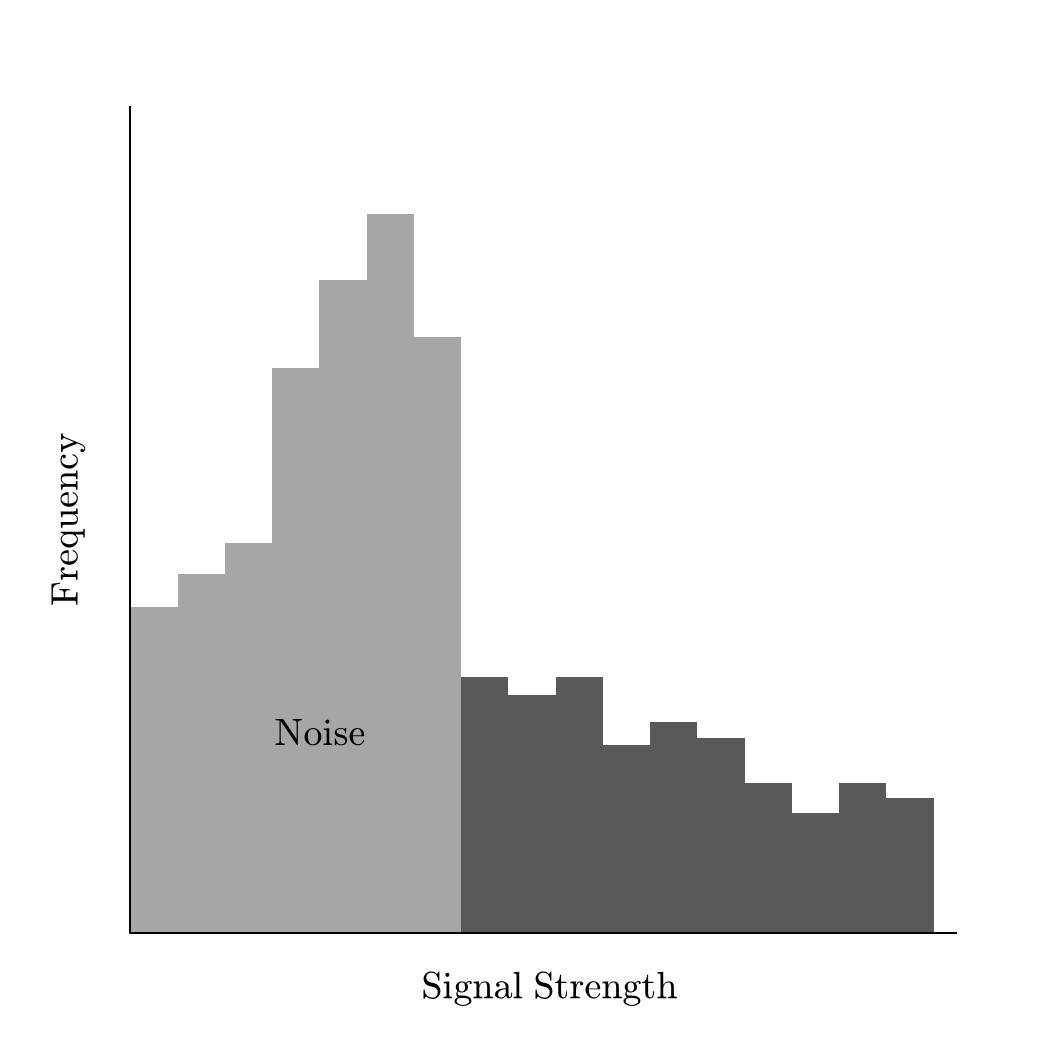
\includegraphics[trim={5 5 5 5},clip]{images/processing-method-signal.jpg}
  \caption{}
  \label{figure:processing:method:signal}
\end{marginfigure}

One of the clues that we can use to estimate the distance between the mobile device and the sensor is the strength of the signal received by the sensor.
The first and obvious way to approach this problem was to try and establish a relationship between the signal strength and distance and to use this to convert the measurement to distance and then set a distance threshold for every location and filter the probe requests which are outside the distance threshold.
However as explained in section \ref{section:uncertainties} this approach was found to not be feasible.
The decay of signal strength with respect to distance is not always constant or linear and in fairly complex to model.
Moreover the parameters with which these two are modelled together such as atmospheric conditions, the presence of obstructions between the source and the target, the material of these obstructions, the strength of the signal (power level) of the source vary widely across locations and across time as well.
This severely limits the ability to establish a simple conversion factor between reported signal strength and distance which makes it important to device a method which takes in to account all of these variables across the various locations.

Assuming that there are specific patterns in a way a sensor is installed at a location, it is expected that the data from around the sensor should reflect these patterns.
That is, in configurations where a specific source of background noise was at a constant distance, there must be a distinct pattern in the number of probe requests reporting signal strength corresponding to that distance.
For example, imagine a sensor in the middle of room such as the initial experiment and there are devices in and outside the room.
In this case, assuming all the devices have roughly similar power levels, there should be a sudden drop in the signal strengths reported by the probe requests generated from outside the room when we look at their frequency distribution.
Alternatively, if there was a stationary source of noise such as a phone shop next to our sensor where hundreds of phones regularly sent probe requests, there should be a sharp rise in the of number of probe requests with reported signal strength corresponding to the distance between the sensor and the phone shop.
Both these sudden changes can be identified by the `breaks' in the distribution of the signal strength data as demonstrated schematically in Figure \ref{figure:processing:method:signal}.
Identification of these breaks in the data could be carried out using traditional one dimensional clustering algorithms such as `jenks natural breaks', `k-means', `quantile' and `hierarchical clustering', etc. which are usually used to find the class intervals in data.
In a simpler cases, the signal strength could be clustered into just `high' and `low' and the probes with low signal strengths could be ignored.

This approach has two primary advantages. 
First is that it does not rely on a predetermined threshold which has to be calculated with a representative sample which is usually not possible in a time series data with such variability.
The second being the methodology should apply for all the variations due to micro site conditions since we are only looking for the relative breaks in the data and not for absolute values.
For example, if the sensor is located inside an enclosure and all the signals are of generally lower strength than usual, this method should still be able to find the distinction between the noise and the data from relatively near the sensors.
The disadvantages of this methods that it might not work with situations where there are multiple sources of noise around the sensor such that they don't create a distinct pattern in their distribution.

\vspace{1.5em}\noindent\textit{Clustering with sequence numbers}\vspace{0.5em}

There have been extensive research carried out on the subject of extracting information about people from Wi-Fi probe requests in the past decade with feasible and favorable results, 
But all of the methods used in the research depends on the Wi-Fi data intrinsically having a primary unique identifier - MAC address.
When the MAC address is removed, or at least rendered non unique, all the previous methods fail and causes significant risk to infrastructure and commercial applications built around Wi-Fi data.
As we briefly saw in Chapter \ref{chapter:literature}, various methods have been devised to overcome this anonymisation process including, but not limited to,
\begin{itemize}[rightmargin=2em, leftmargin=2em]
  \itemsep-0.25cm
  \item \textit{Profiling Manufacturers}: estimating the device model information from a known dataset of manufacturers and device behaviours \citep{martin2016}
  \item \textit{Scrambler attack}: using another small part of the physical layer specification for Wi-Fi \citep{vo2016, bloessl2015}
  \item \textit{Timing attack}: where the packet sequence information along with information elements present in the probe request frame is used \citep{matte2016, cheng2016}. 
\end{itemize}

A combination of these methodologies has been even proven to produce de-anonymised globally unique device information \cite[-4cm]{vanhoef2016, martin2017}. 
Though these approaches are effective, some times even up to 90\%, they usually result in serious risk of breach of privacy of the users of the mobile devices by revealing their MAC addresses or crosses ethical lines by tricking the devices to send more information than it includes in the probe requests.
Moreover these risks are considered as vulnerabilities by the computer security industry and are usually `patched' in a reasonable amount of time hence reducing their effectiveness in long term.
This led the research to explore methodologies for estimating the number of unique mobile devices from a set of anonymised probe requests, without the need to reveal their original device information.

Although sequence number of the packet is not strictly unique to a mobile device, we hypothesize that we can use them to estimate the number of unique devices.
\citet{vanhoef2016} used optional information present in the probe requests - Information Elements (IE) along with the sequence numbers to successfully fingerprint the devices.
This approach has become increasingly difficult as mobile phone manufacturers, especially Apple, have severely limited the number of information elements in the probe requests to curb such finger printing process.
This problem affects the established commercial solutions using Wi-Fi probe requests such as Blix, Walkbase, Euclid Analytics, RetailNext etc. who solve it by combining the Wi-Fi data with other suite of data such as Cameras, Lasers or infra red counters which doesn't apply for our research.
Recently another solution to this problem have been proposed where the authors tried to solve the similar problem using a \textit{Hidden Markov Models} based trajectory inference algorithm \cite{hong2018}.
Unfortunately the scope of such methods was limited to enclosed, exit controlled public spaces such as shopping malls, railway stations, etc. and did not translates well to open retail high streets essentially led the research to devise a novel method to suit the context.

The first obvious approach taken was to establish a `factor of randomisation' - a ratio of total number of randomised probe requests emitted to the number of unique MAC addresses in them.
This factor was then used to adjust the counts when aggregating randomised probe requests.
As explained in section \ref{section:uncertainties} the rate of probe request generation is highly variable and this approach which assumes a constant and stable rate of probe requests was found to be not feasible.
Moreover since the software and specification change frequently, this method was found to not work in the long term.
There needs to be a more general approach which was independent of the device model or manufacturer.

\begin{marginfigure}
  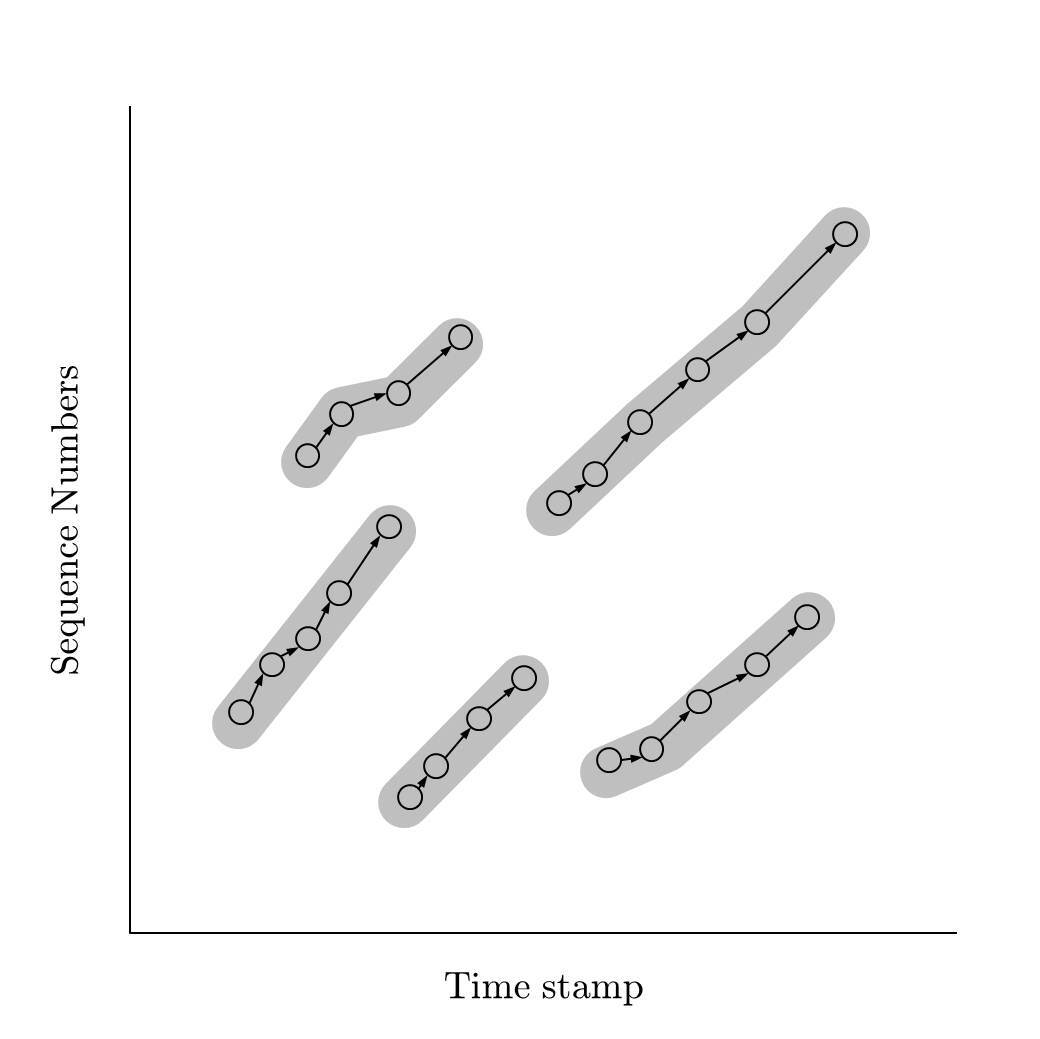
\includegraphics[trim={5 5 5 5}, clip]{images/processing-method-sequence.jpg}
  \caption{}
  \label{figure:processing:method:sequence}
\end{marginfigure}

From our initial experiments explained in section \ref{section:intial:experiments}, it was found that OUI and the sequence number of the probe request were the most promising information to achieve this.
It was also noticed that the sequence numbers when plotted against time stamps show distinct streak patterns which could be isolated as single unique devices.
The logic is that since we can receive only one probe request at one time, the sequence numbers and timestamps increase for a set of probe requests generated from an unique device we can link them up using a graph based algorithm as illustrated in Figure \ref{figure:processing:method:sequence}.
Such algorithm would create a graph with the randomised probe requests where the nodes were the probe requests themselves and the edges were created between them based on the following rules:

\begin{enumerate}[rightmargin=3em, leftmargin=3em] 
  \itemsep-0.5em
  \item A link could go only forward in time.
  \item A link could go from low to high sequence numbers. 
  \item A link could exist between nodes with a maximum time difference of $\alpha$ - time threshold.
  \item A link could exist between nodes with a maximum sequence number difference of $\beta$ - sequence threshold.
  \item A node could have only one incoming link and one outgoing link, which is the shortest of all such possible links.
\end{enumerate}

The first two rules arise from how the Wi-Fi data collection process works.
The third and fourth rules creates a kind of 2 dimensional moving window within which all the links are connected. 
The finally rule simplifies the graph into strands of unique devices based on the assumption that closest points within the window should belong together.
This, of course, will not work accurately when there are intersections between these strands.
This problem could be made more accurate by calculate angular changes similar to techniques used in creating `dual networks' in roads \cite{masucci2014} but could disproportionately increase the amount of processing needed.
Hence for this research the former method which uses the shortest link was used.

After simplifying the graph, conceptually, each connected component corresponds to a device generating probe requests periodically with increasing sequence numbers.
A unique identification number could be then assigned to the nodes based on the connected component of the graph they belonged to.
This unique identifier can be then used in the place of MAC addresses for aggregation of the anonymised probe requests.
As discussed in section \ref{wifi-as-source-of-data}, the sequence numbers are not always increasing, they get reset after 4096 thus this method can lead to multiple unique identifiers being reported for a single device.
This could be potentially solved by treating sequence numbers as a `ratio' scale while calculating distances between probe requests.
Since a sample consisting of randomised probe requests sent by "Google" devices in the data collected from the initial experiments showed that only 0.5\% of the sample had their sequence number reset in a given period, this effect has been deemed inconsequential and ignored in this research.

\vspace{1.5em}\noindent\textit{Calibrating with Ground Truth}\vspace{0.5em}

Since proportions of mobile device ownership was an external uncertainty to this study and could arise from variety of spatio - temporal and demographic factors, the study aimed to solve the uncertainty by using a manual sample count at each location.
An adjustment factor or an `offset' was calculated for each location by comparing the sensor-based counts and ground truth similar what was done in the beginning of the project.
This adjustment factor was was then used to adjust the rest of the data reliably to reflect the ground truth in absolute numbers.
On a project with a large scope such as Smart Street Sensor, this calibration not only applies on top of the methodologies increasing their accuracy, they can be carried out periodically at chosen locations to improve the quality of the estimation over time.

These three methods together provides a unified methodology for converting the Wi-Fi probe requests into footfall.
But these methods need empirical experiments for a successful implementation with real-world data.
For example, the signal strength methodology we need to find the most suitable one dimensional clustering algorithm and for the sequencing method the values of threshold need to be calculated.
These questions were answered by applying the methods on the data collected in the experiments and pilot study as detailed in the upcoming sections.

%-------------------------------------------------------------------------------%
\subsection{Oxford Street Experiment}
%-------------------------------------------------------------------------------%

The primary aim of the initial experiment conducted at Oxford street, London was to collect data to validate the filtering and clustering methods against the scale and complexity of an open public area such as a retail high street.
It was also aimed at finding the algorithm which was best suited for the one dimensional classification of signal strengths as 'low' and 'high' in order to filter out the background noise.

The first step was to create a base line count or `raw count' without any cleaning procedures where the probe requests were aggregated  by just their MAC addresses for every minute.
This generated a continuous, minute by minute count of the number of people estimated to be near the sensor where it is assumed that each MAC address corresponded to a mobile device and hence a pedestrian.
This preliminary `footfall' count was then compared to the actual number of pedestrians recorded manually to check for it's robustness.
The statistic - Mean Absolute Percentage Error (MAPE) as a measure of robustness of the count, since it provided a simple and quick idea of how much the two time series data differed from each other.
Though this MAPE generally doesn't work with datasets with significant number of data points which are not known or contains any zero values, because of the busy nature of the survey location there were no such intervals without any footfall.

It was observed that the MAPE in these raw counts when compared to the actual ground truth was around 425\%.
This confirmed the presence of large amount of noise in the data which may have been generated by the sources of uncertainties discussed in section \ref{section:uncertainties} as observed in the previous experiments and it also demonstrating the need for filtering the data before aggregating them into footfall.
 
\begin{table}
  \footnotesize
  \caption{Comparison of clustering algorithms with a sample of 40000 probe requests}
  \centering
  \begin{tabular}{lcc} 
    \toprule
     Algorithm				      	& Time (s)& MAPE\\
    \midrule
     Quantile				        	& 0.002 	&  27 \% \\
     K-Means			 	        	& 0.007 	& -23 \% \\
     Hierarchical Clustering	& 172.520	&  -9 \% \\
     Bagged Clustering 		  	& 0.135 	& -30 \% \\
     Fisher 				        	& 3.034 	& -30 \% \\
     Jenks Natural Break 	   	& 556.279	& -30 \% \\
     \bottomrule
  \end{tabular}
  \label{table:processing:oxst:classification}
\end{table}

These prone requests were then classified as `high signal strength' and `low signal strength' using various one dimensional clustering algorithms.
The algorithms used were as k-means, quantile, hierarchical clustering, bagged clustering, fisher and jenks natural breaks with the number of clusters set as 2.
Due to the processor intensive nature of some of these algorithms only a sample of 40,000 probe requests were selected for this benchmarking exercise.
For each exercise the resulting probe requests were filtered only for the ones with high signal strength and rest were discarded.
Like earlier the filtered probe requests are then converted into footfall counts by aggregating them based on their MAC addresses and compared to the manual footfall counts.

Two metrics were collected for each clustering algorithm - the time it took to classify all the data points in the sample and the amount of MAPE in the resulting footfall estimates.
The results are shown in Table \ref{table:processing:oxst:classification}.
It was found that out of all algorithms,  hierarchical clustering and jenks natural break provided the least amount of errors.
However these two algorithms were designed to identify class intervals in a dataset normally uses for datasets much smaller datasets and were extremely resource intensive for practical use with a larger dataset.
It was also found that k-means algorithm gave the quickest results with the lowest MAPE, closely followed by quantile algorithm.
The cut-off point or threshold for the collected data with which we could classify the probe requests as high and low was found to be -71 dBm using the k-means algorithm.
When the data were aggregated after this filtration process removing all the probes with 'low' signal strength, it resulted in a footfall count with a MAPE of 30\%.
This was extremely encouraging considering the magnitude of improvement but it was still not completely evident that this filtering process is indeed just removing noise from outside or if it has any kind independence from the configuration of sensor at the location.
These concerns need to be addressed with a larger survey with multiple locations as discussed in the pilot study.

\begin{figure*}
  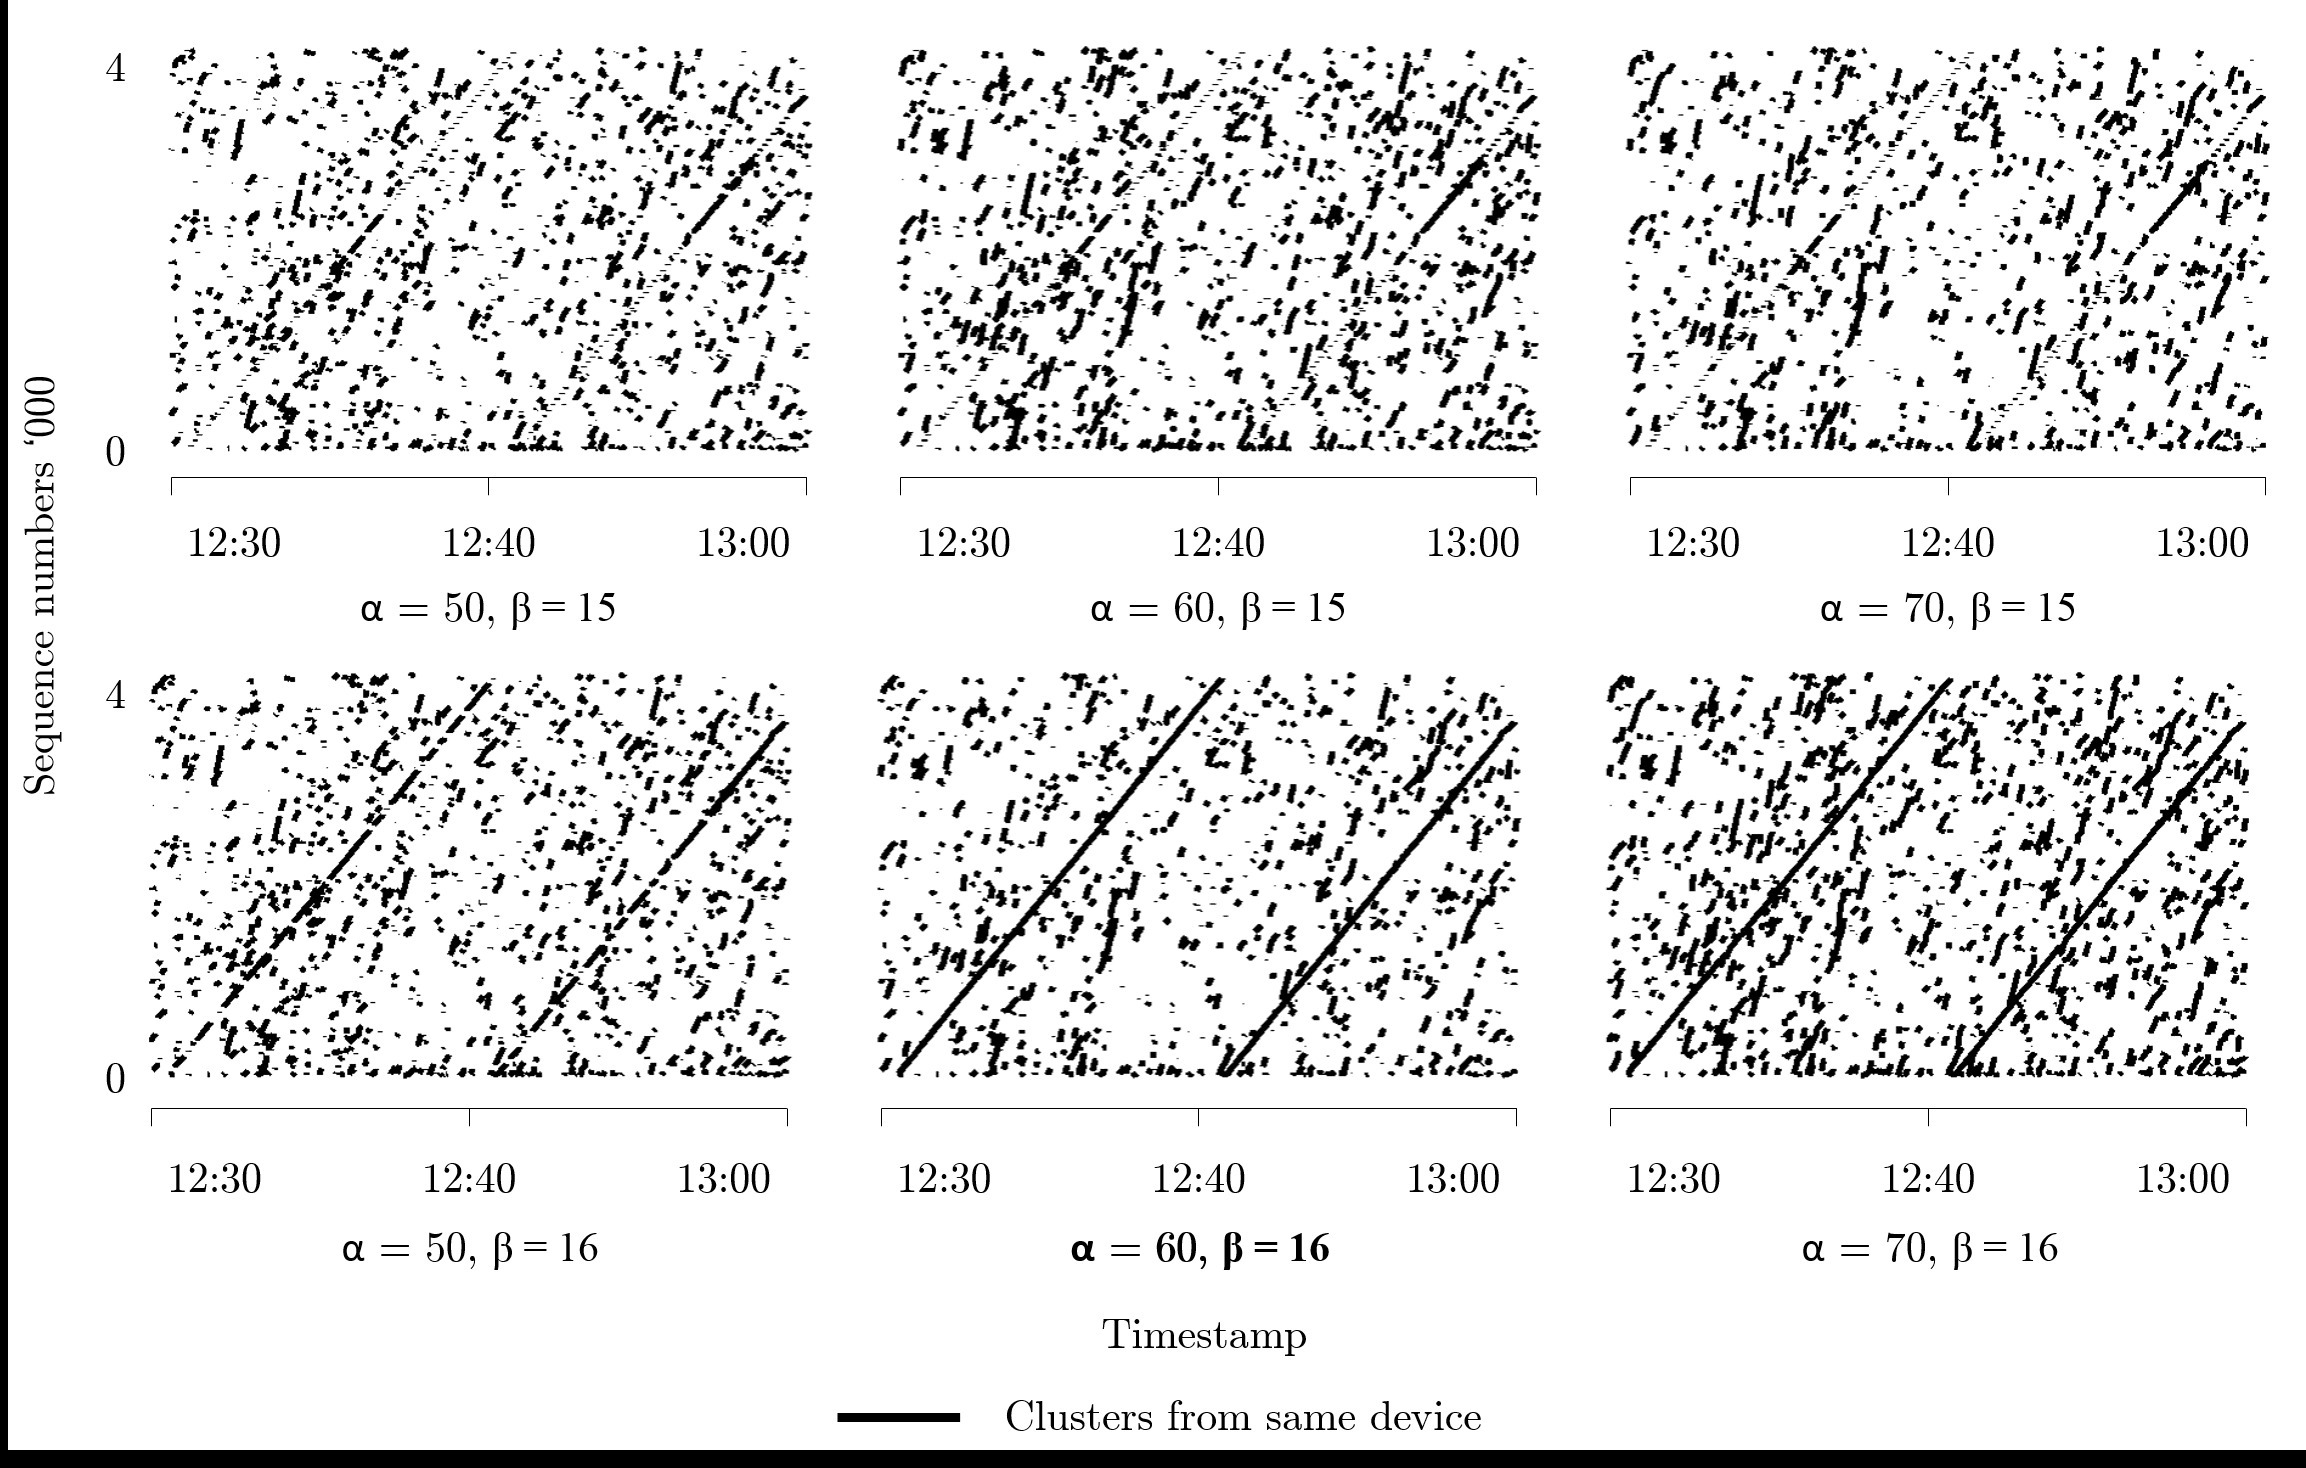
\includegraphics[trim={1 1 1 1},clip]{images/processing-oxst-clusters.jpg}
  \caption{}
  \label{figure:processing:oxst:clusters}
\end{figure*}

With the filtering method validated, the next step was to identify the probe requests which are generated by the same device irrespective of the MAC randomisation using their sequence numbers.
The graph theory based algorithm defined earlier was employed and each local probe request was assigned an alternative unique identifier or signature independent of their the MAC addresses.
Since a baseline for the nature or frequency of the MAC address randomisation process could not be established, the surveyor's mobile device was used as a reference.
As the surveyor's device was being actively used to count pedestrians with it's Wi-Fi module kept active without establishing connection to any network it was known that the device was continuously probing for new networks.
Moreover since the screen of the device was switched on with constant taps the frequency of these probe requests were also more than normal.
It was also known that the OUI of the device corresponds to the vendor - 'Google' and the device was regularly randomising it's MAC address, thus providing us an excellent reference with which we could determine if the clustering method has worked.

\begin{figure}
  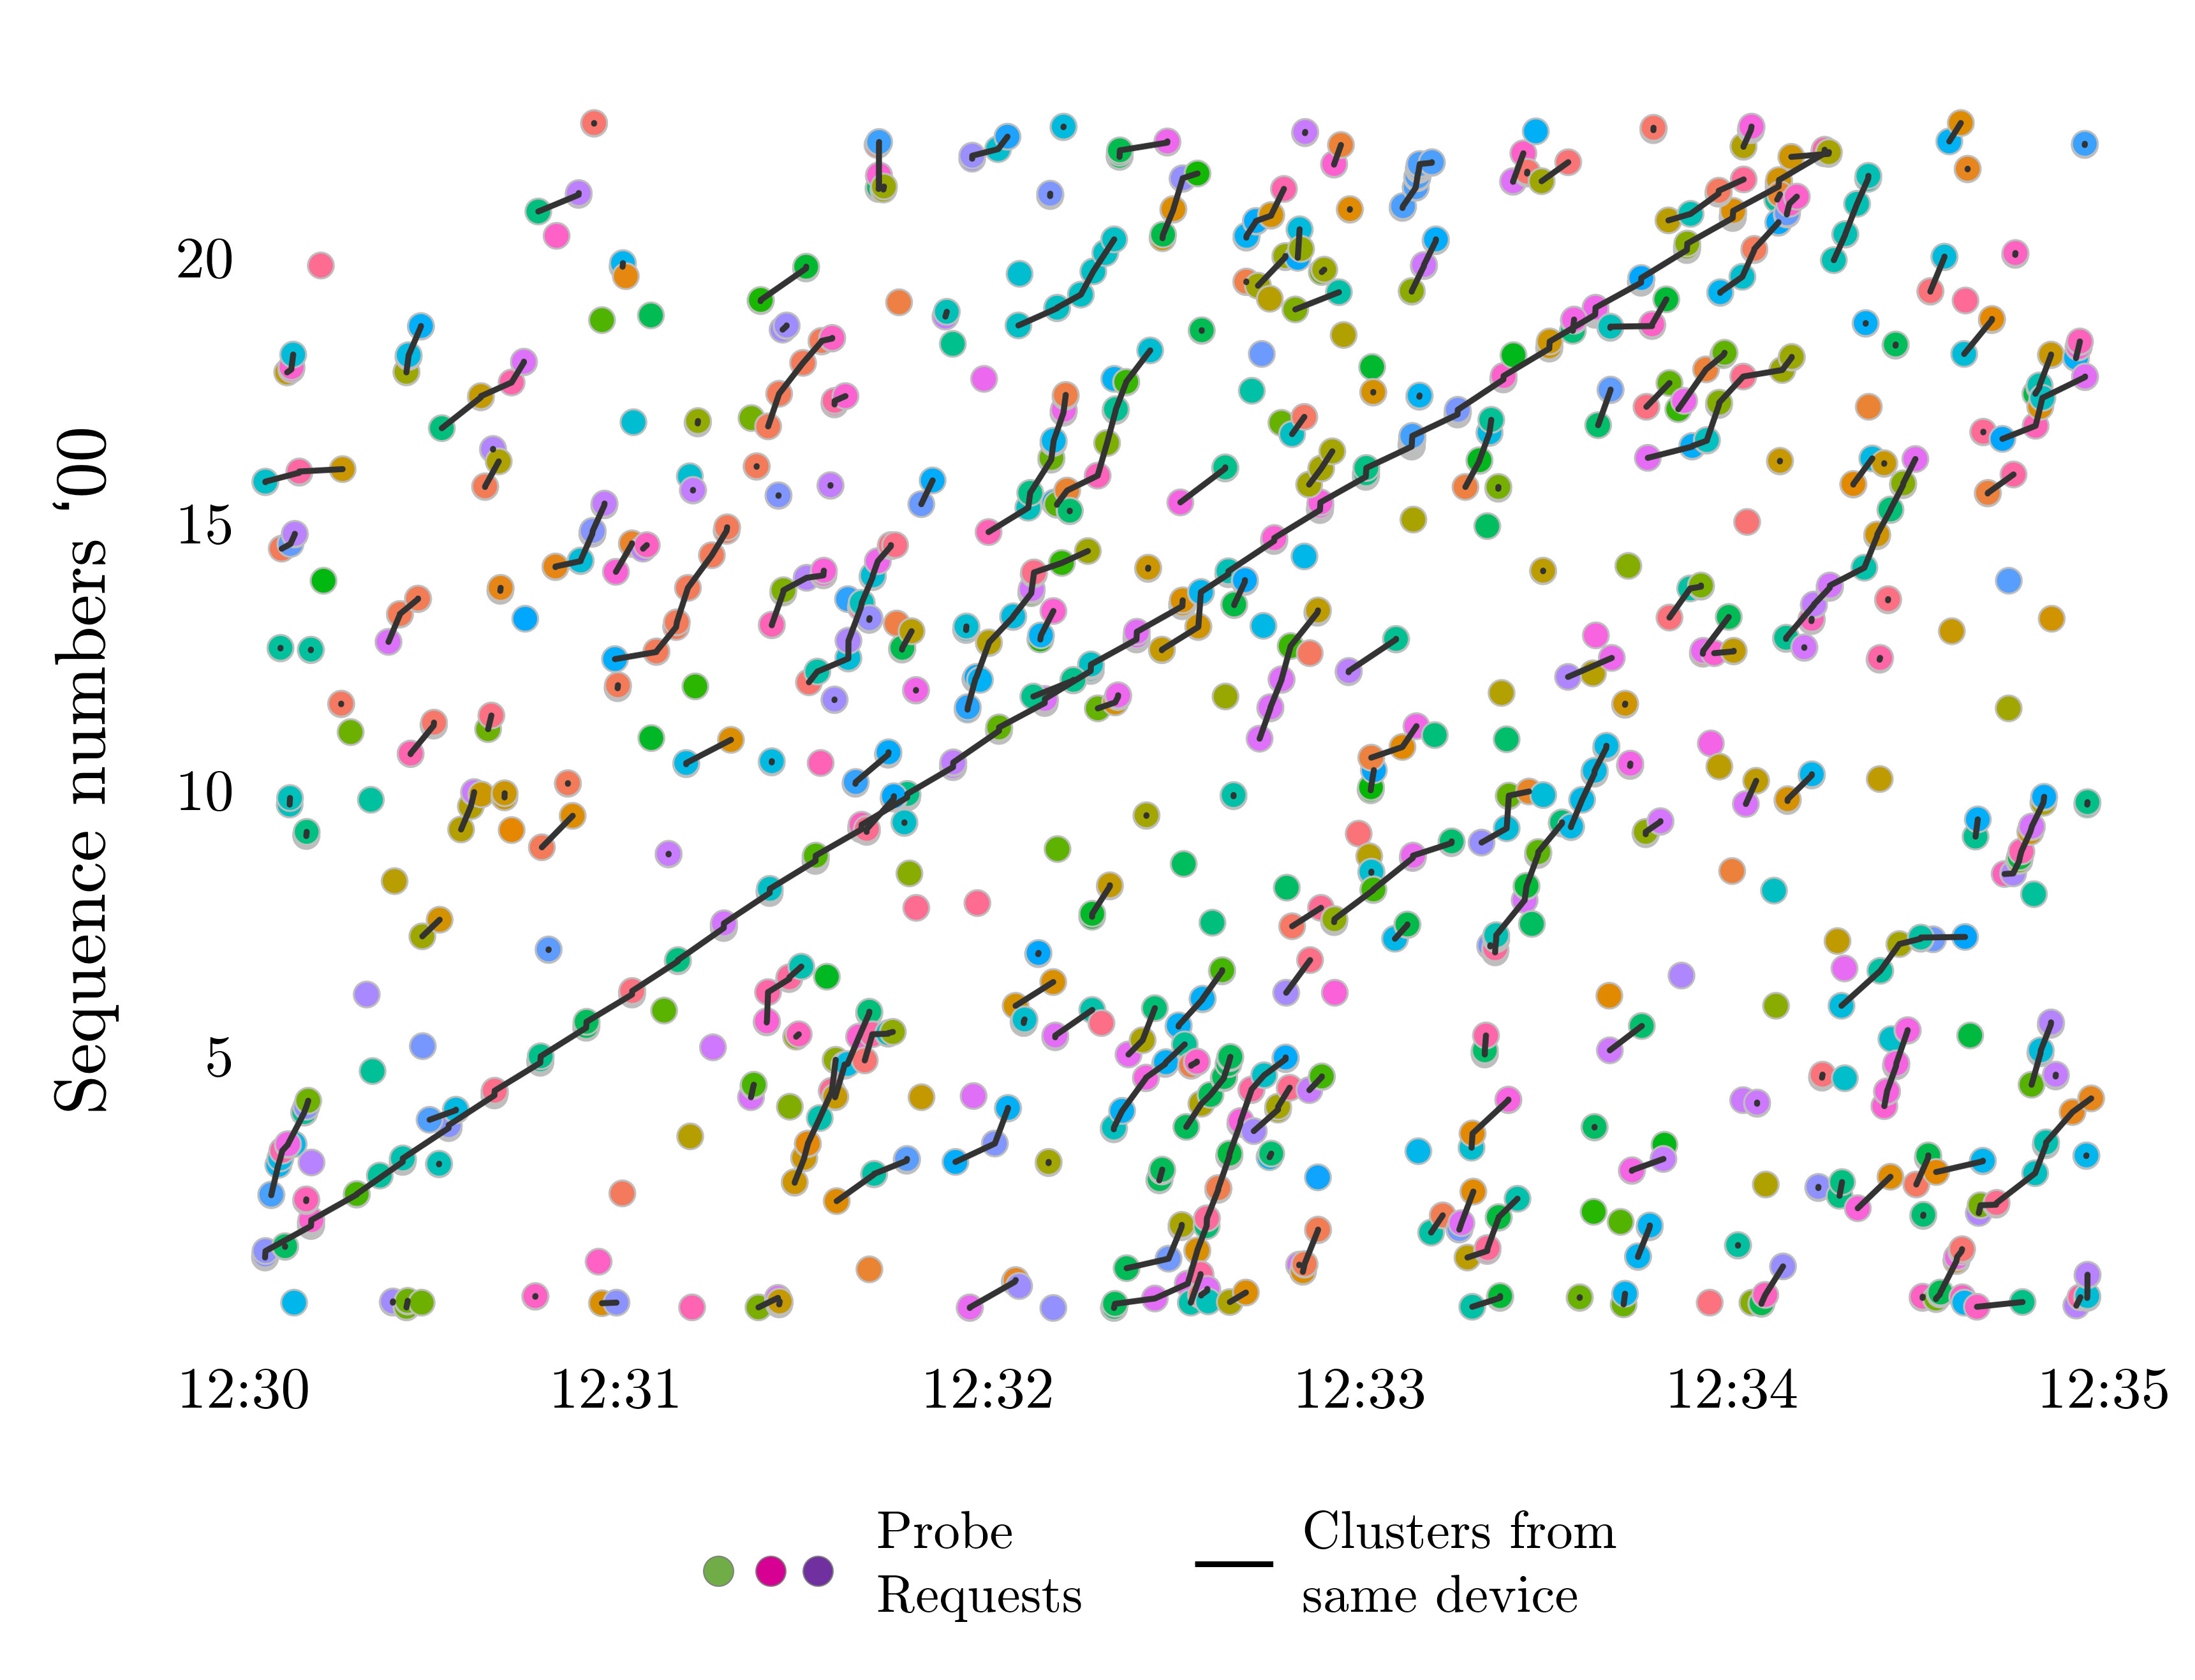
\includegraphics[trim={3 3 3 3},clip]{images/processing-oxst-fingerprinting.jpg}
  \caption{test}
  \label{figure:processing:oxst:fingerprinting}
\end{figure}

The algorithm required two parameters which needs to be determined empirically - sequence threshold and time threshold which was done using a trial and error as described below.
The clustering process was done repeatedly with increasing values for both the thresholds in steps of 1 and for each step the resulting clusters were examined to see if the data from reference device were clustered into one device.
The minimum possible time and sequence thresholds at which the algorithm clusters the reference device properly without over clustering the other probe requests or under clustering as multiple devices.
This process is illustrated in Figure \ref{figure:processing:oxst:clusters} where it can be observed that the threshold for time $\alpha$ and the threshold for sequence numbers, $\beta$ are 16 seconds and 60 respectively.

Figure \ref{figure:processing:oxst:fingerprinting} shows the results of this clustering process on a small set of randomised probe requests collected in this experiment.
The probe requests with different randomised MAC address are shown by the coloured dots and the lines joining them show that those probe requests were clustered together by the algorithm and are most likely be generated by the same device.
The data were finally aggregated like before but with this device signature rather than local MAC addresses resulting in a footfall count with a MAPE of -18\% compared to the manual count.
It is important to notice that this clustering was undertaken on top the filtering done based on signal strength, and only for the probe requests with randomised MAC addresses.
A comparison of minute by minute counts resulting from different filtering processes along with the ground truth is shown in Figure \ref{figure:processing:oxst:results} illustrating the promising effectiveness of the methods.

\begin{figure}
  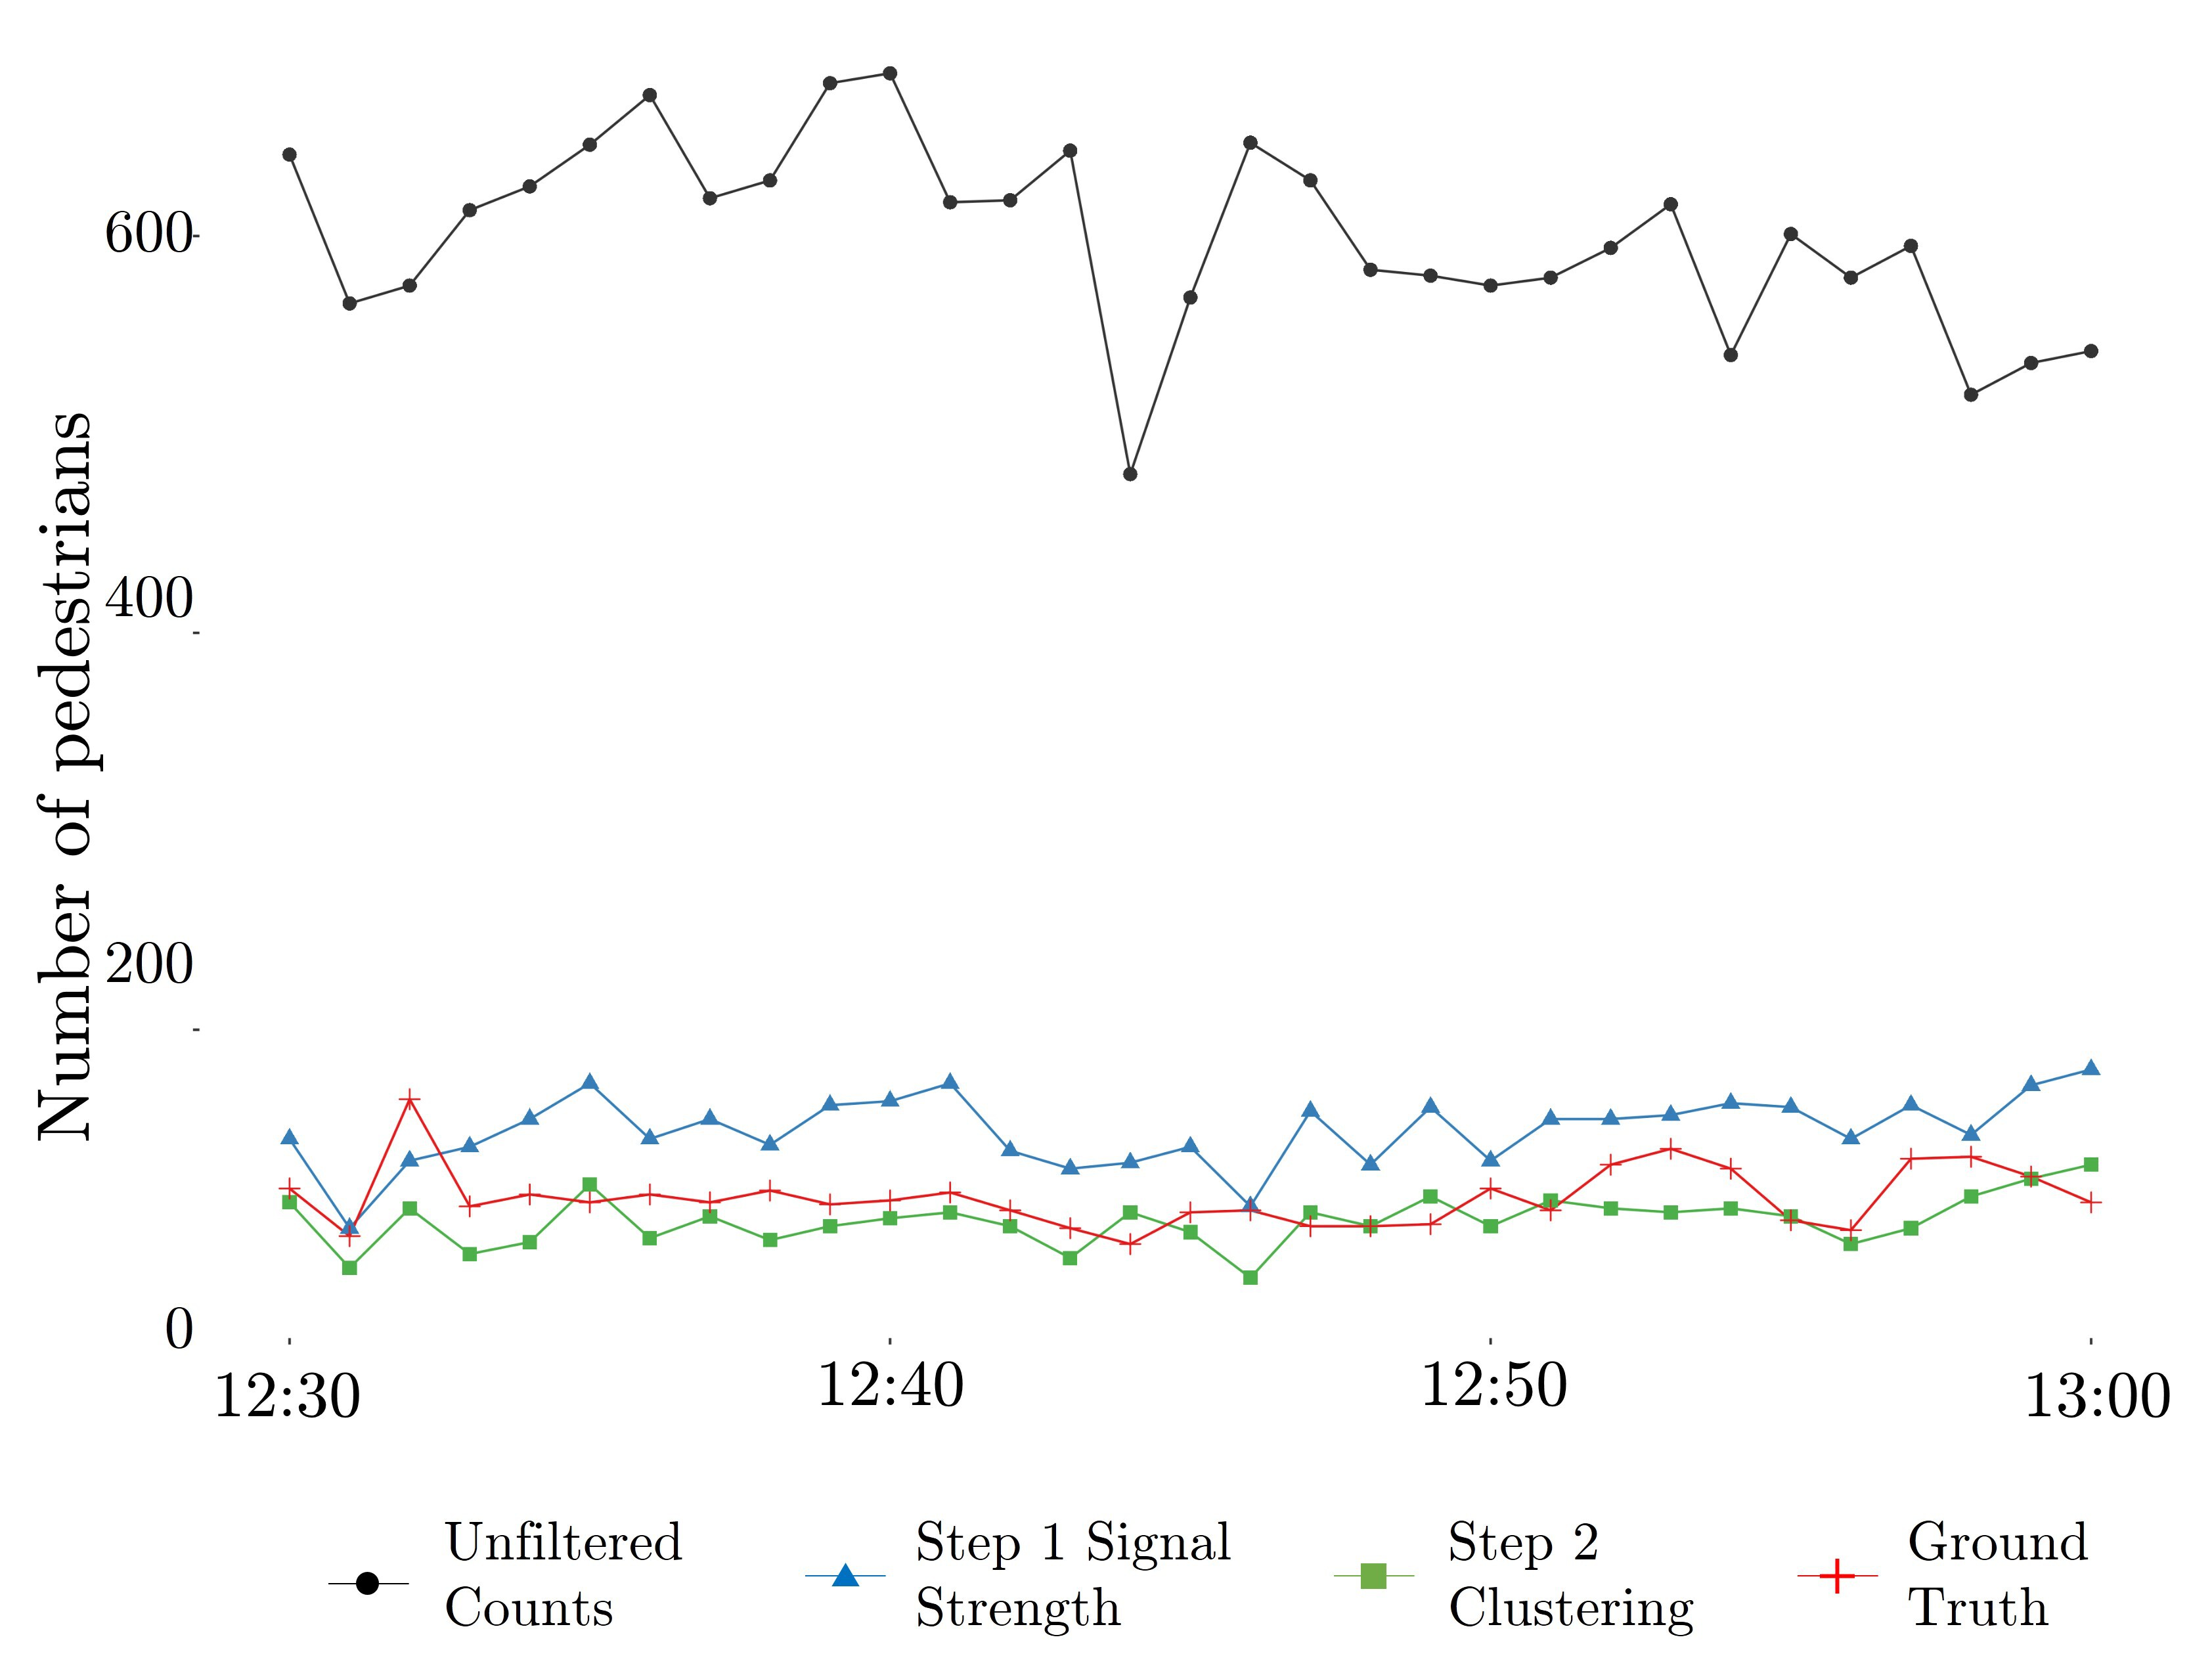
\includegraphics[trim={3 3 3 3},clip]{images/processing-oxst-results.jpg}
  \caption{test}
  \label{figure:processing:oxst:results}
\end{figure}

To summarise, the data from initial experiments suggest that both the filtering using signal strength and the clustering using sequence numbers worked well on complex real world data and resulted in fairly accurate pedestrian counts with a MAPE of 20\%.
It was also found that `k-means' and `quantile' are best algorithms for clustering signal strengths and the optimum thresholds for time and sequence numbers for the clustering algorithm were around 16 and 60 respectively.

%-------------------------------------------------------------------------------%
\subsection{Pilot Study}
%-------------------------------------------------------------------------------%

With encouraging results from the initial experiment, the next step was to check if the methods work on various locations where sensors were installed in different configurations using the data from the pilot study.
The distribution of the signal strengths of all the probe requests collected at each locations were created and were compared to the corresponding sensor configurations at these locations.
These when visualised as density plots as shown in Figure \ref{figure:processing:pilot:signal}, show a clear relation between the distribution of the signal strength and the distance and complexity of the source of noise at each location.
It was observed that when there is clear distinction between the source of noise where stationary devices were generating randomised local probe requests, the signal strength distribution shows a clear distinction between high and low values.
For example, location 5 where the noise is generated by a phone shop next door, a significant spike in the number of probe requests generated with similar low signal strength was also reported.
Whereas, location 2 - a restaurant located next to a public square with seating on both sides of the sensor shows no such discernible distinction of any sort.
This demonstrates that the filtering using signal strength works but at the same time depends heavily on the assumption that the sensor is installed in such a way that the field of measurement is clearly `visible' in terms of distance from it.`
Figure \ref{figure:processing:pilot:signal} confirmed the intuition that data collected at location 2 and 4 would be harder to clean than the ones collected at locations 1, 3 and 5.
The signal strength threshold, calculated using k-means algorithm, for all the locations except for 2 were between -72 dBm and -70 dBm - very much in line with the findings of the initial experiment.
This also introduced the possibility that -70dBm could be used as a rule of thumb for filtering noise at a general location unless it faces specific challenges like location 2.
It is important to note that as the aim was to compare the counts with manual counts, the data used to calculate the threshold pertains only the time when manual counting was undertaken at these locations.
Like before, the data were aggregated using MAC addresses after removing points with low signal strength and compared with manual counts and the results are shown in Table \ref{table:processing:pilot:results}.
In this exercise probe requests with MAC addresses which were repeating within a same 15 minute window were also removed.

\begin{figure*}
  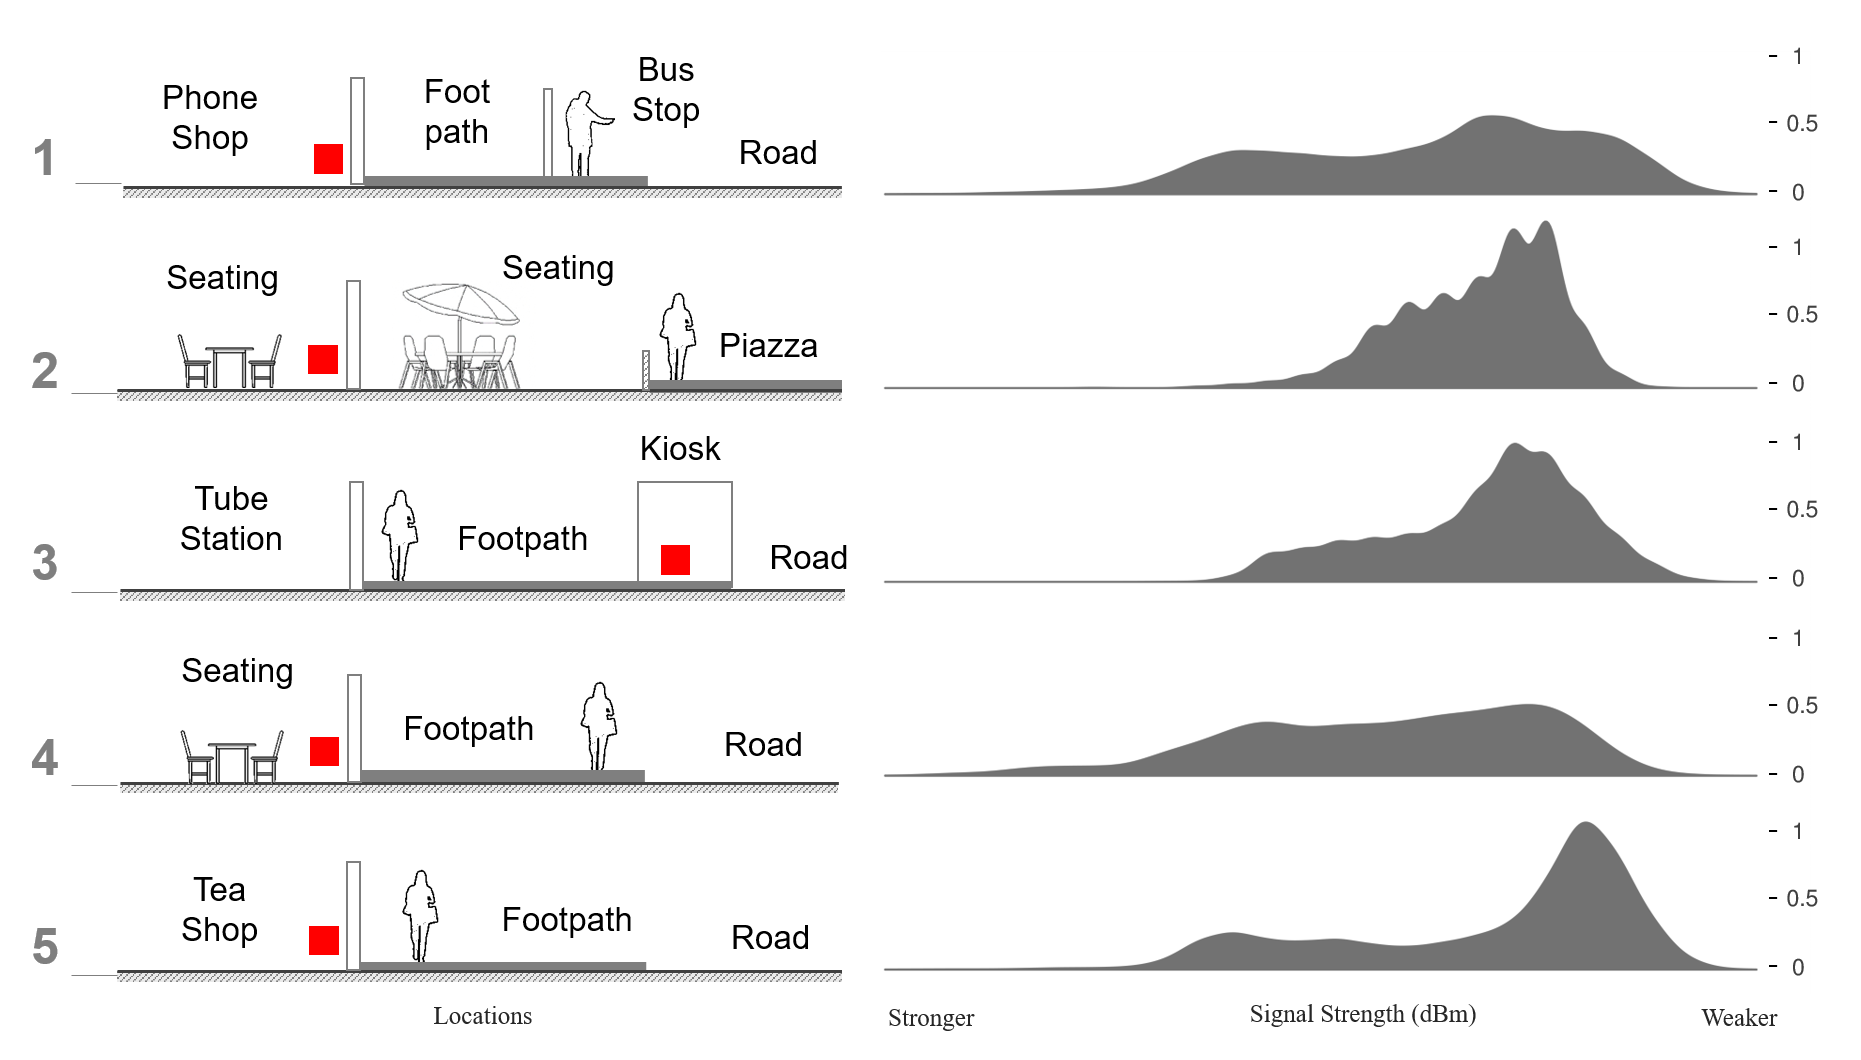
\includegraphics{images/processing-pilot-signal.png}
  \caption{}
  \label{figure:processing:pilot:signal}
\end{figure*}

We observed that the MAPE at location 1,4 and 5 which were reduced to -19\% to 150\% from the original 250\% to 500\% making this an ideal candidate for quick and easy cleaning procedure for most practical applications.
Location 2 and 3 were found to be particularly tricky while former had the propensity to overestimate the footfall the latter underestimated the same.
This could also be attributed the configuration of the sensor at the particular location.
Location 3 was particularly interesting as it is the only location with no source of stationary noise and almost all the probe requests collected at the location should be coming from genuine footfalls.
We can observe that the filtering needs to be less aggressive in locations without any obvious source of noise to prevent underestimating footfall at these locations.

\begin{centering}
\begin{table}
\footnotesize
\caption{Results of footfall estimation at each location as Mean Absolute Percentage Error (MAPE) after each step of the filtering process}
{\begin{tabular}{ccccccc} 
\toprule
& Signal    & Adjustment & MAPE      & MAPE      & MAPE       & MAPE final \\
Sensor  & threshold & factor     & before    & after     & after    & adjusted\\
& (-dBm)    &            & filtering & filtering & clustering & count\\
&           &            & (\%)      & (\%)      & (\%)       & (\%)\\
\midrule
1 & -70 & 1.25 & 259 &  22 & -13 &  9 \\
2 & -74 & 0.51 & 928 & 396 & 206 & 55 \\
3 & -72 & 1.60 &  87 & -19 & -31 & 10 \\
4 & -70 & 0.88 & 498 & 142 &  52 & 33 \\
5 & -72 & 0.80 & 473 &  84 &  38 & 11 \\
\bottomrule
\end{tabular}}
\label{table:processing:pilot:results}
\end{table}
\end{centering}

The next step was to test the sequence number based clustering algorithm on these location. 
The sequence numbers clustering algorithm was run on the local MAC addresses to cluster the probe requests and the resulting device signatures were used to aggregate them into footfall counts. 
The results showed that this process further reduced the MAPE to almost 13\% - 300\% on all the sensors with a clean configuration.
Location 3 and 2 were still outliers among all the others due to their complex configurations. Finally step was to test the simple manual calibration process where an adjustment factor was calculated for each location as the ratio between footfall estimated from the sensor after all the processing and the actual pedestrian counts and this factor is used to adjust the counts.
It is important to note that the adjustment and MAPE were calculated by using one of the intervals where the manual counts were carried out at a location on other intervals.
This process further reduces the MAPE to 10 - 50\% while taking care of the over-counting problem in Location 3.
Location 2 is still not accurate as the MAPE after all the processing that were being done showing the limitation of the methods discussed.
Figure \ref{figure:processing:pilot:final} shows the effectiveness of these cleaning procedures at each location.

To summarise, the pilot study confirmed the findings from the initial experiment by showing that the signal strength based filtering is effective and provides a quick and easy way to clean out the noise along with the sequence numbers based finger-printing technique.
It also demonstrated that the sensors with no discernible stationary source of noise tend to under-count pedestrians and requires the calibration is done using manually collected data while sensors with seating next to them over-count significantly.
However, the study also proved that through whole process of cleaning the errors can be reduced substantially and get the sensor based counts accurate within 10\% of the ground truth.

\begin{figure*}
  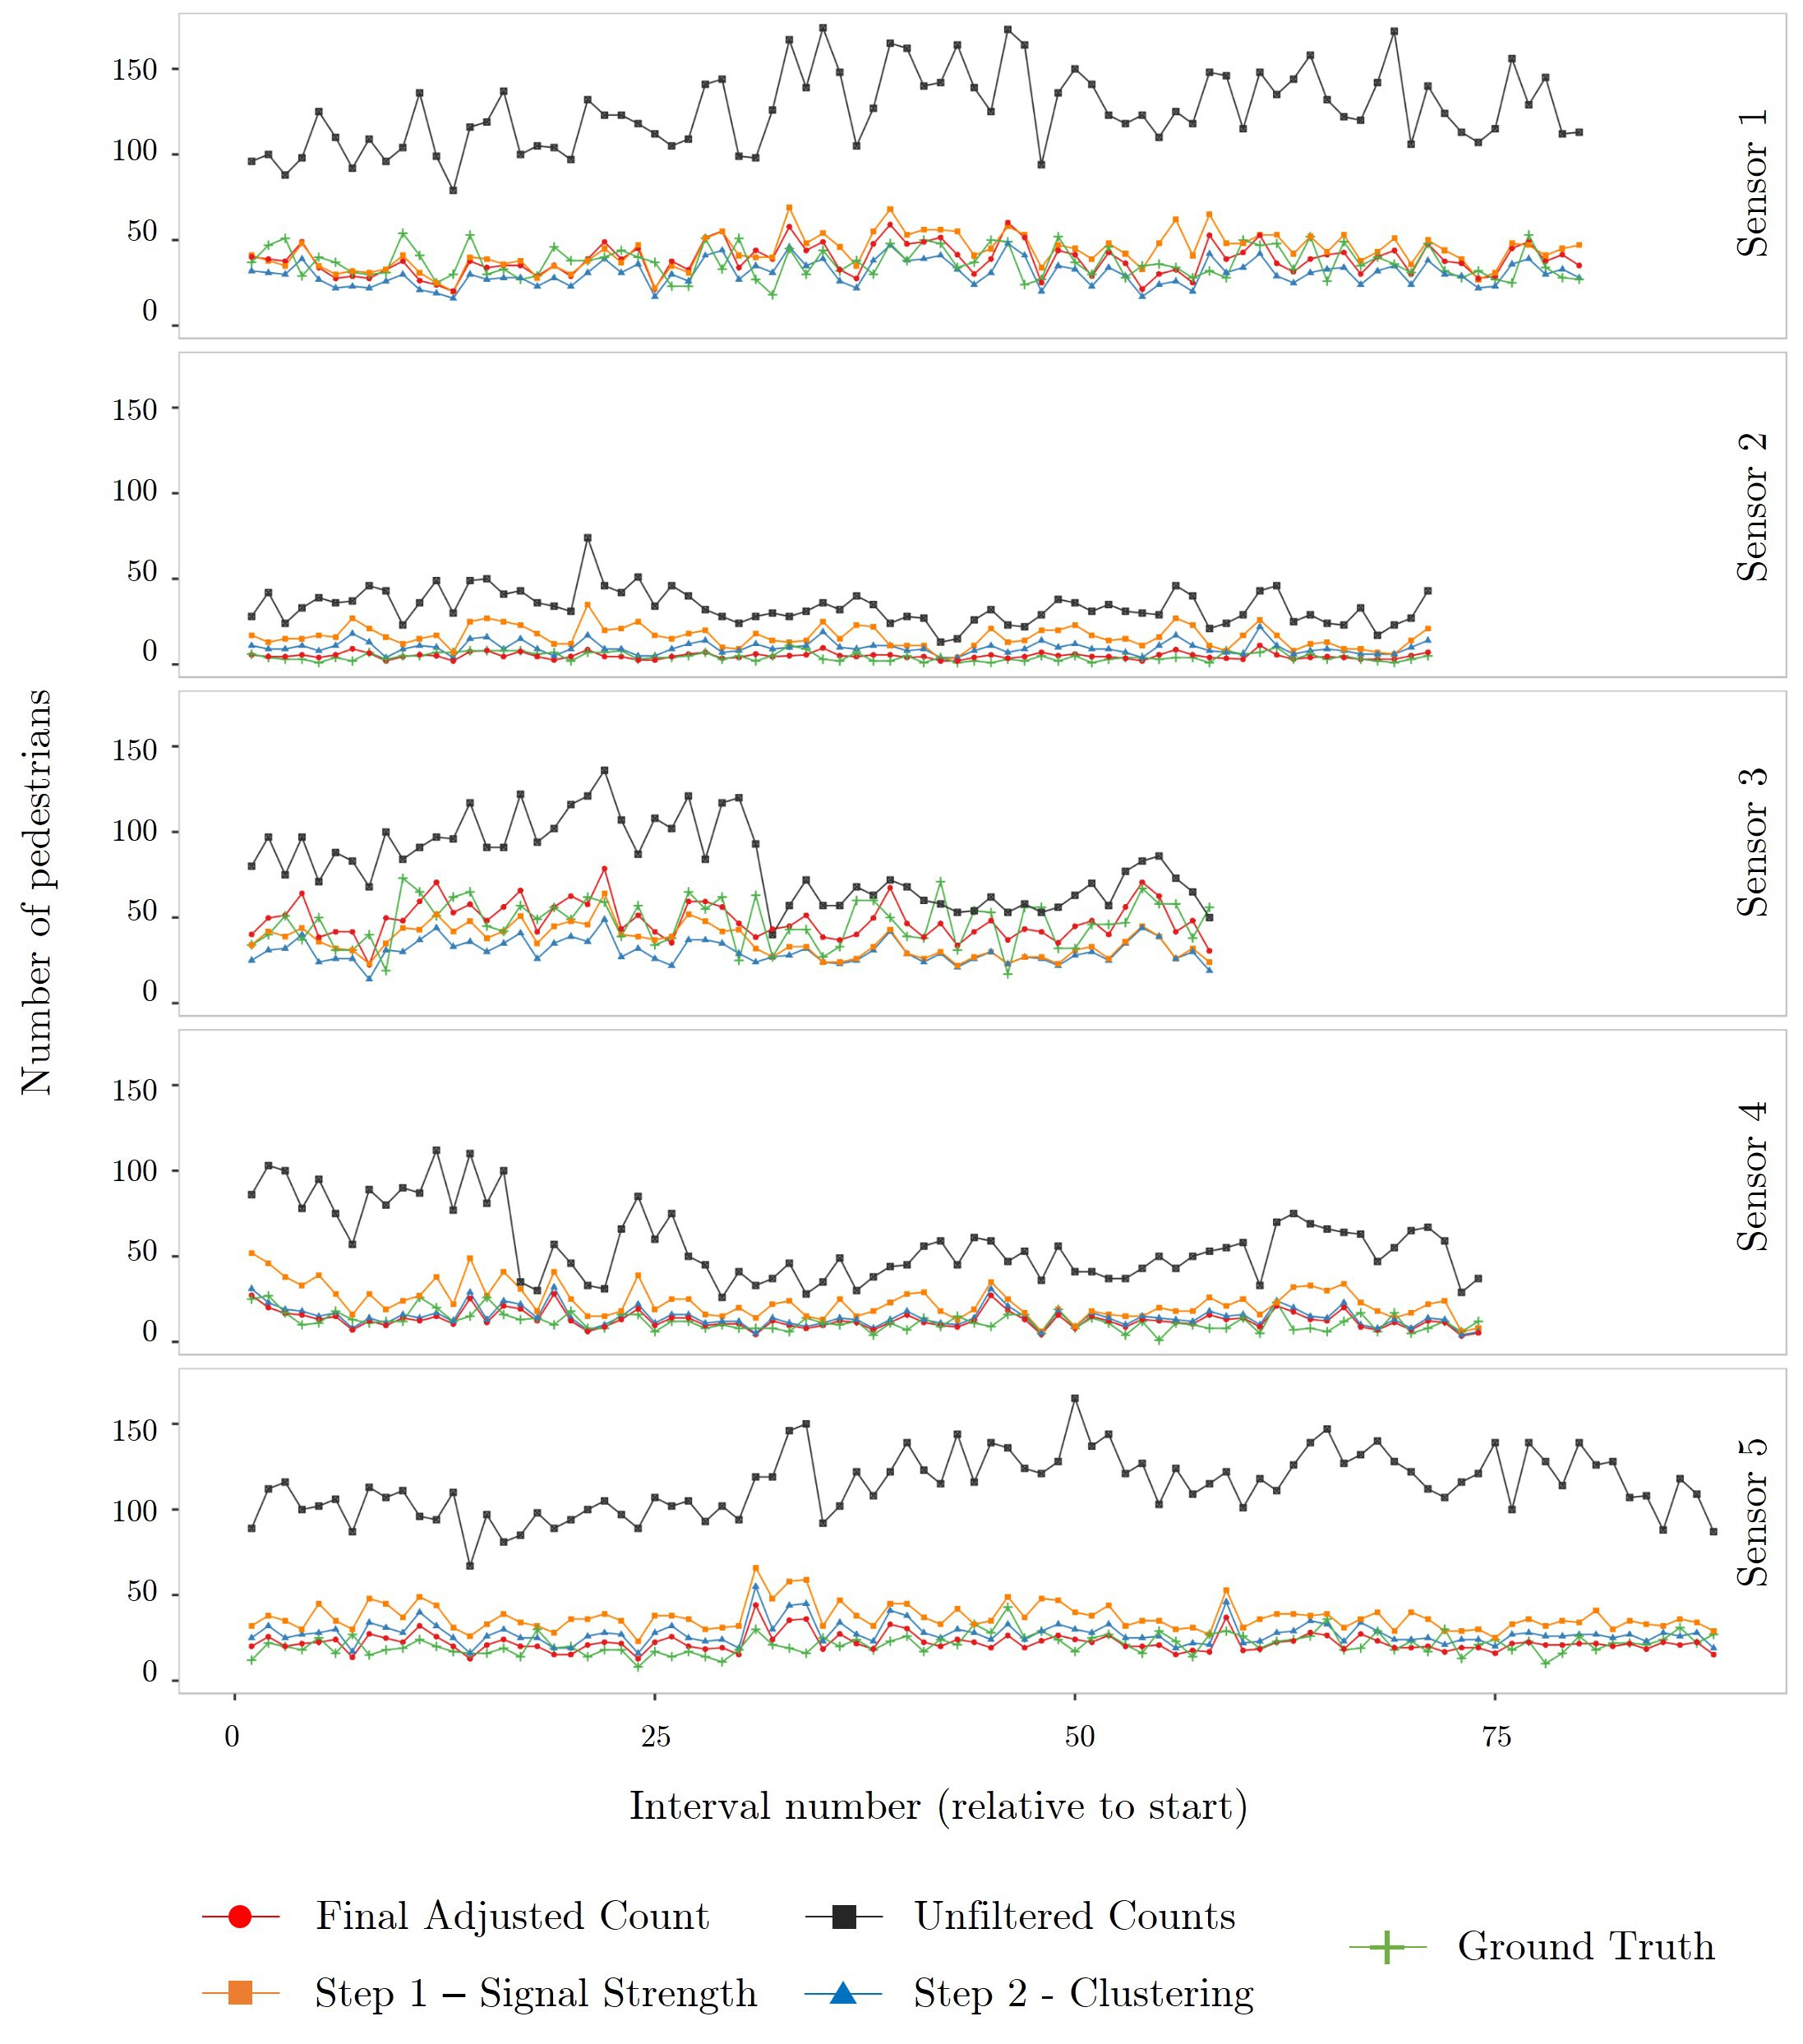
\includegraphics[trim=6 6 6 6, clip]{images/processing-pilot-results.jpg}
  \caption{Comparison of the filtering process with the ground truth in all the locations.}
  \label{figure:processing:pilot:final}
\end{figure*}

%-------------------------------------------------------------------------------%
\subsection{Smart Street Sensor Project}
%-------------------------------------------------------------------------------%
In addition to solving the problems arising due to privacy oriented decisions and figuring out methods to enhance Wi-Fi based analysis, one of the primary objectives of the research was to solve the problem faced by the Smart Street Sensor project with the explosion of MAC randomisation.
The number of probe requests and unique MAC addresses nearly tripled in one week in the fall of 2017 essentially making the data unusable and adding extreme risks to the projects feasibility.
The methodologies discussed above would be perfect for the SSS project and when implemented it could improved the project's long term feasibility immensely.
However, being designed from a commercial point of view by the data partner, the SSS project's implementation poses significant challenges in adapting the methods as well.

\begin{itemize}[rightmargin=2em,leftmargin=2em]
  \item \textit{Lack of data} - The data collected by the SSS project is optimised for transferring large amount of data with the least possible cost and hence the project collects only the fields which are extremely important. For example, sequence number, Information elements, SSID, etc. are not available in the dataset.
  \item \textit{Aggregation} - To further optimise the size of the data transfer the data points are aggregated at the device level every five minutes. Hence the time information has a resolution of 5 minutes and the signal strength of packets with same MAC addresses were summarised to either the maximum or minimum values observed in that interval.
  \item \textit{Cost} - When changing the design of the project and the major challenge faced the cost that was associated with every change. For example, due to the size of the project, changing the amount of data transferred even marginally translates into a significant cost in terms of internet bandwidth or when introducing a large change in the project also involves cost in terms of development, testing, deployment and testing.
\end{itemize}

The above challenges make the sequence number based clustering impossible with the data available through SSS sensors and only the signal strength based filtering could be applied. 
Even the signal strengths do not have the same granular information in them as the pilot study which greatly affects output of the k-means algorithm as shown in Figure \ref{figure:processing:sss:signals}
Nevertheless, an attempt was made to use the signal strength based filtering of the data generated from the SSS sensors.
The data collected at the location where the pilot studies were conducted along with manual counting were extracted out of the SSS project and the filtering methodology is applied to them.
Since we only have the minimum signal strength for all the probe requests that were compressed, they were weighted using the total number of probes that constitute the aggregated packet.
%200 words about the signal comparison

\begin{figure}
  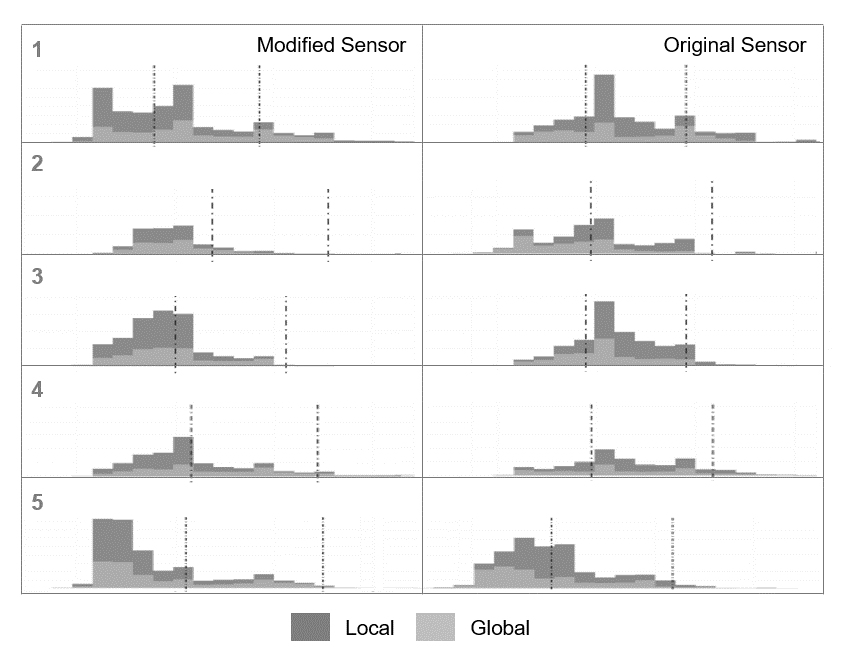
\includegraphics[trim={5 5 5 5}, clip]{images/processing-sss-signals.png}
  \caption{Comparison of the filtering process with the ground truth in all the locations.}
  \label{figure:processing:sss:signals}
\end{figure}

%200 words about the counts comparison and how our methodology fails 
These filtered data were then aggregated by MAC addresses and compared to other counts as shown in Figure \ref{figure:processing:sss:comparison}. 

\begin{figure*}
  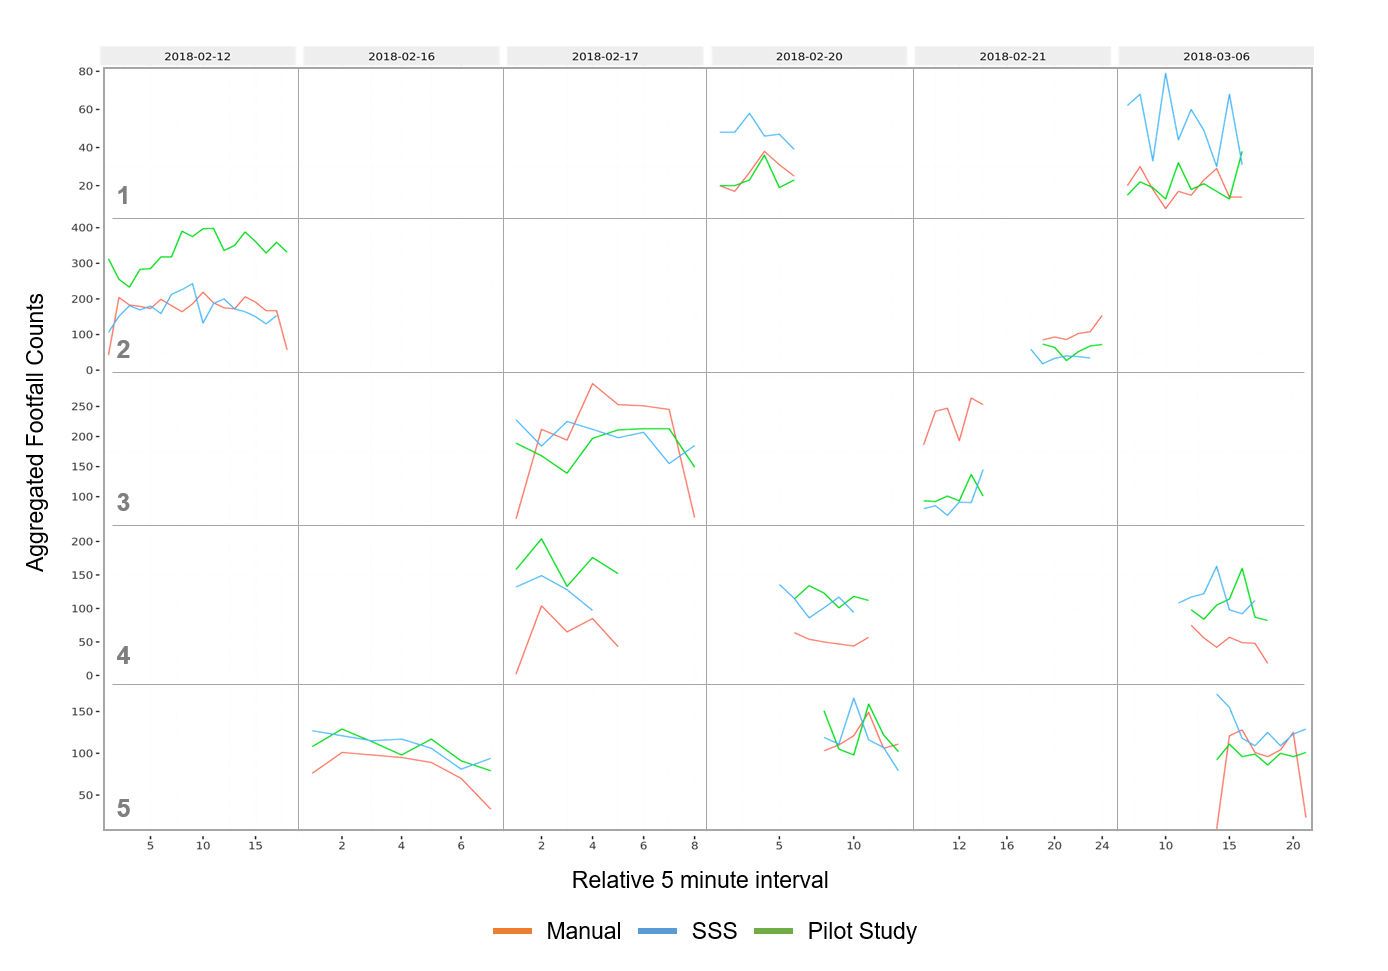
\includegraphics[trim={10 10 33 10}, clip]{images/processing-sss-comparison.png}
  \caption{Comparison of the filtering process with the ground truth in all the locations.}
  \label{figure:processing:sss:comparison}
\end{figure*}

\vspace{1.5em}\noindent\textit{A simple \& effective solution}\vspace{0.5em}

%-------------------------------------------------------------------------------%
\subsection{Discussion}
%-------------------------------------------------------------------------------%

